\documentclass[9pt,a4paper]{report}
\usepackage{mwe}
\usepackage{listings}
\usepackage{amsmath}
\usepackage{graphicx}
\usepackage{subfig}
\usepackage{float}
\usepackage{xcolor}
\usepackage{multirow}
\usepackage{hyperref}
\usepackage{fancyhdr}
\usepackage{sectsty}
\usepackage[dvipsnames]{xcolor}
\usepackage{soul}
\usepackage[compact]{titlesec}
\usepackage{float}
\usepackage[left=0.5cm,right=0.5cm,top=0.5cm,bottom=0.5cm]{geometry}
\graphicspath{{Report/Part 1.1}{Report/Part 1.1/Series Forward-Bias Diode Circuit}{Report/Part 1.2}{Report/Part 1.2/Series Reverse-breakdown Zener Diode Circuit}{Report/Part 1.3}{Report/Part 1.3/Parallel Opposing Polarities Diode Circuit}{Report/Part 1.3/Series Opposing Polarities Zener Diode Circuit}{Report/Part 1.4}{Report/Part 1.4/Full Rectifier circuits/Bridge With Filter}{Report/Part 1.4/Full Rectifier circuits/Bridge With Zener}{Report/Part 1.4/Full Rectifier circuits/Full Wave Bridge}}

\newcommand*{\nchapter}[1]{%
	\chapter*{#1}%
	\addcontentsline{toc}{chapter}{#1}
	\vspace{-14mm}}
\newcommand*{\nsection}[1]{%
	\section*{#1}%
	\addcontentsline{toc}{section}{#1}}
\newcommand*{\nsubsection}[1]{%
	\subsection*{#1}%
	\addcontentsline{toc}{subsection}{#1}}
\newcommand*{\nsubsubsection}[1]{%
	\subsubsection*{#1}%
	\addcontentsline{toc}{subsubsection}{#1}}

\chaptertitlefont{\large}
\sectionfont{\normalsize}
\fontsize{9}{11}\selectfont
\begin{document}
	\begin{titlepage}
		\centering
		\vspace*{1.5in}
		
\includegraphics[width=0.15\textwidth]{W-Logo_Purple_RGB}\par\vspace{1cm}
		{\LARGE \textsc{University of Washington}\par}
		\vspace{1cm}
		{\Large \textsc{BEE331 Lab 3}\par}
		\vspace{1.5cm}
		{\huge\bfseries \par}
		\vspace{2cm}
		{\Large\itshape 2301991\hspace{55pt}2130474\par}
		{\Large\itshape Jason Truong\hspace{31pt}Henry Haight\par}
		\vfill
		supervised by\par
		Prof.~Joseph \textsc{Decuir}
		\date{2024\\ January}
		\vfill
		% Bottom of the page
		{\large \today\par}
		\vspace*{1.5in}
	\end{titlepage}



\nchapter{CMOS NAND Gate}
\nsection{Design Objective}
In this section we use the CD4007 IC pakage as a NAND logic gate then testing it with two inputs to create a truth table for the transistors.

\nsection{Circuit Design Outline}
\begin{figure}[hp!]
	\centering
	\subfloat[\centering NAND Circuit Transistors]{{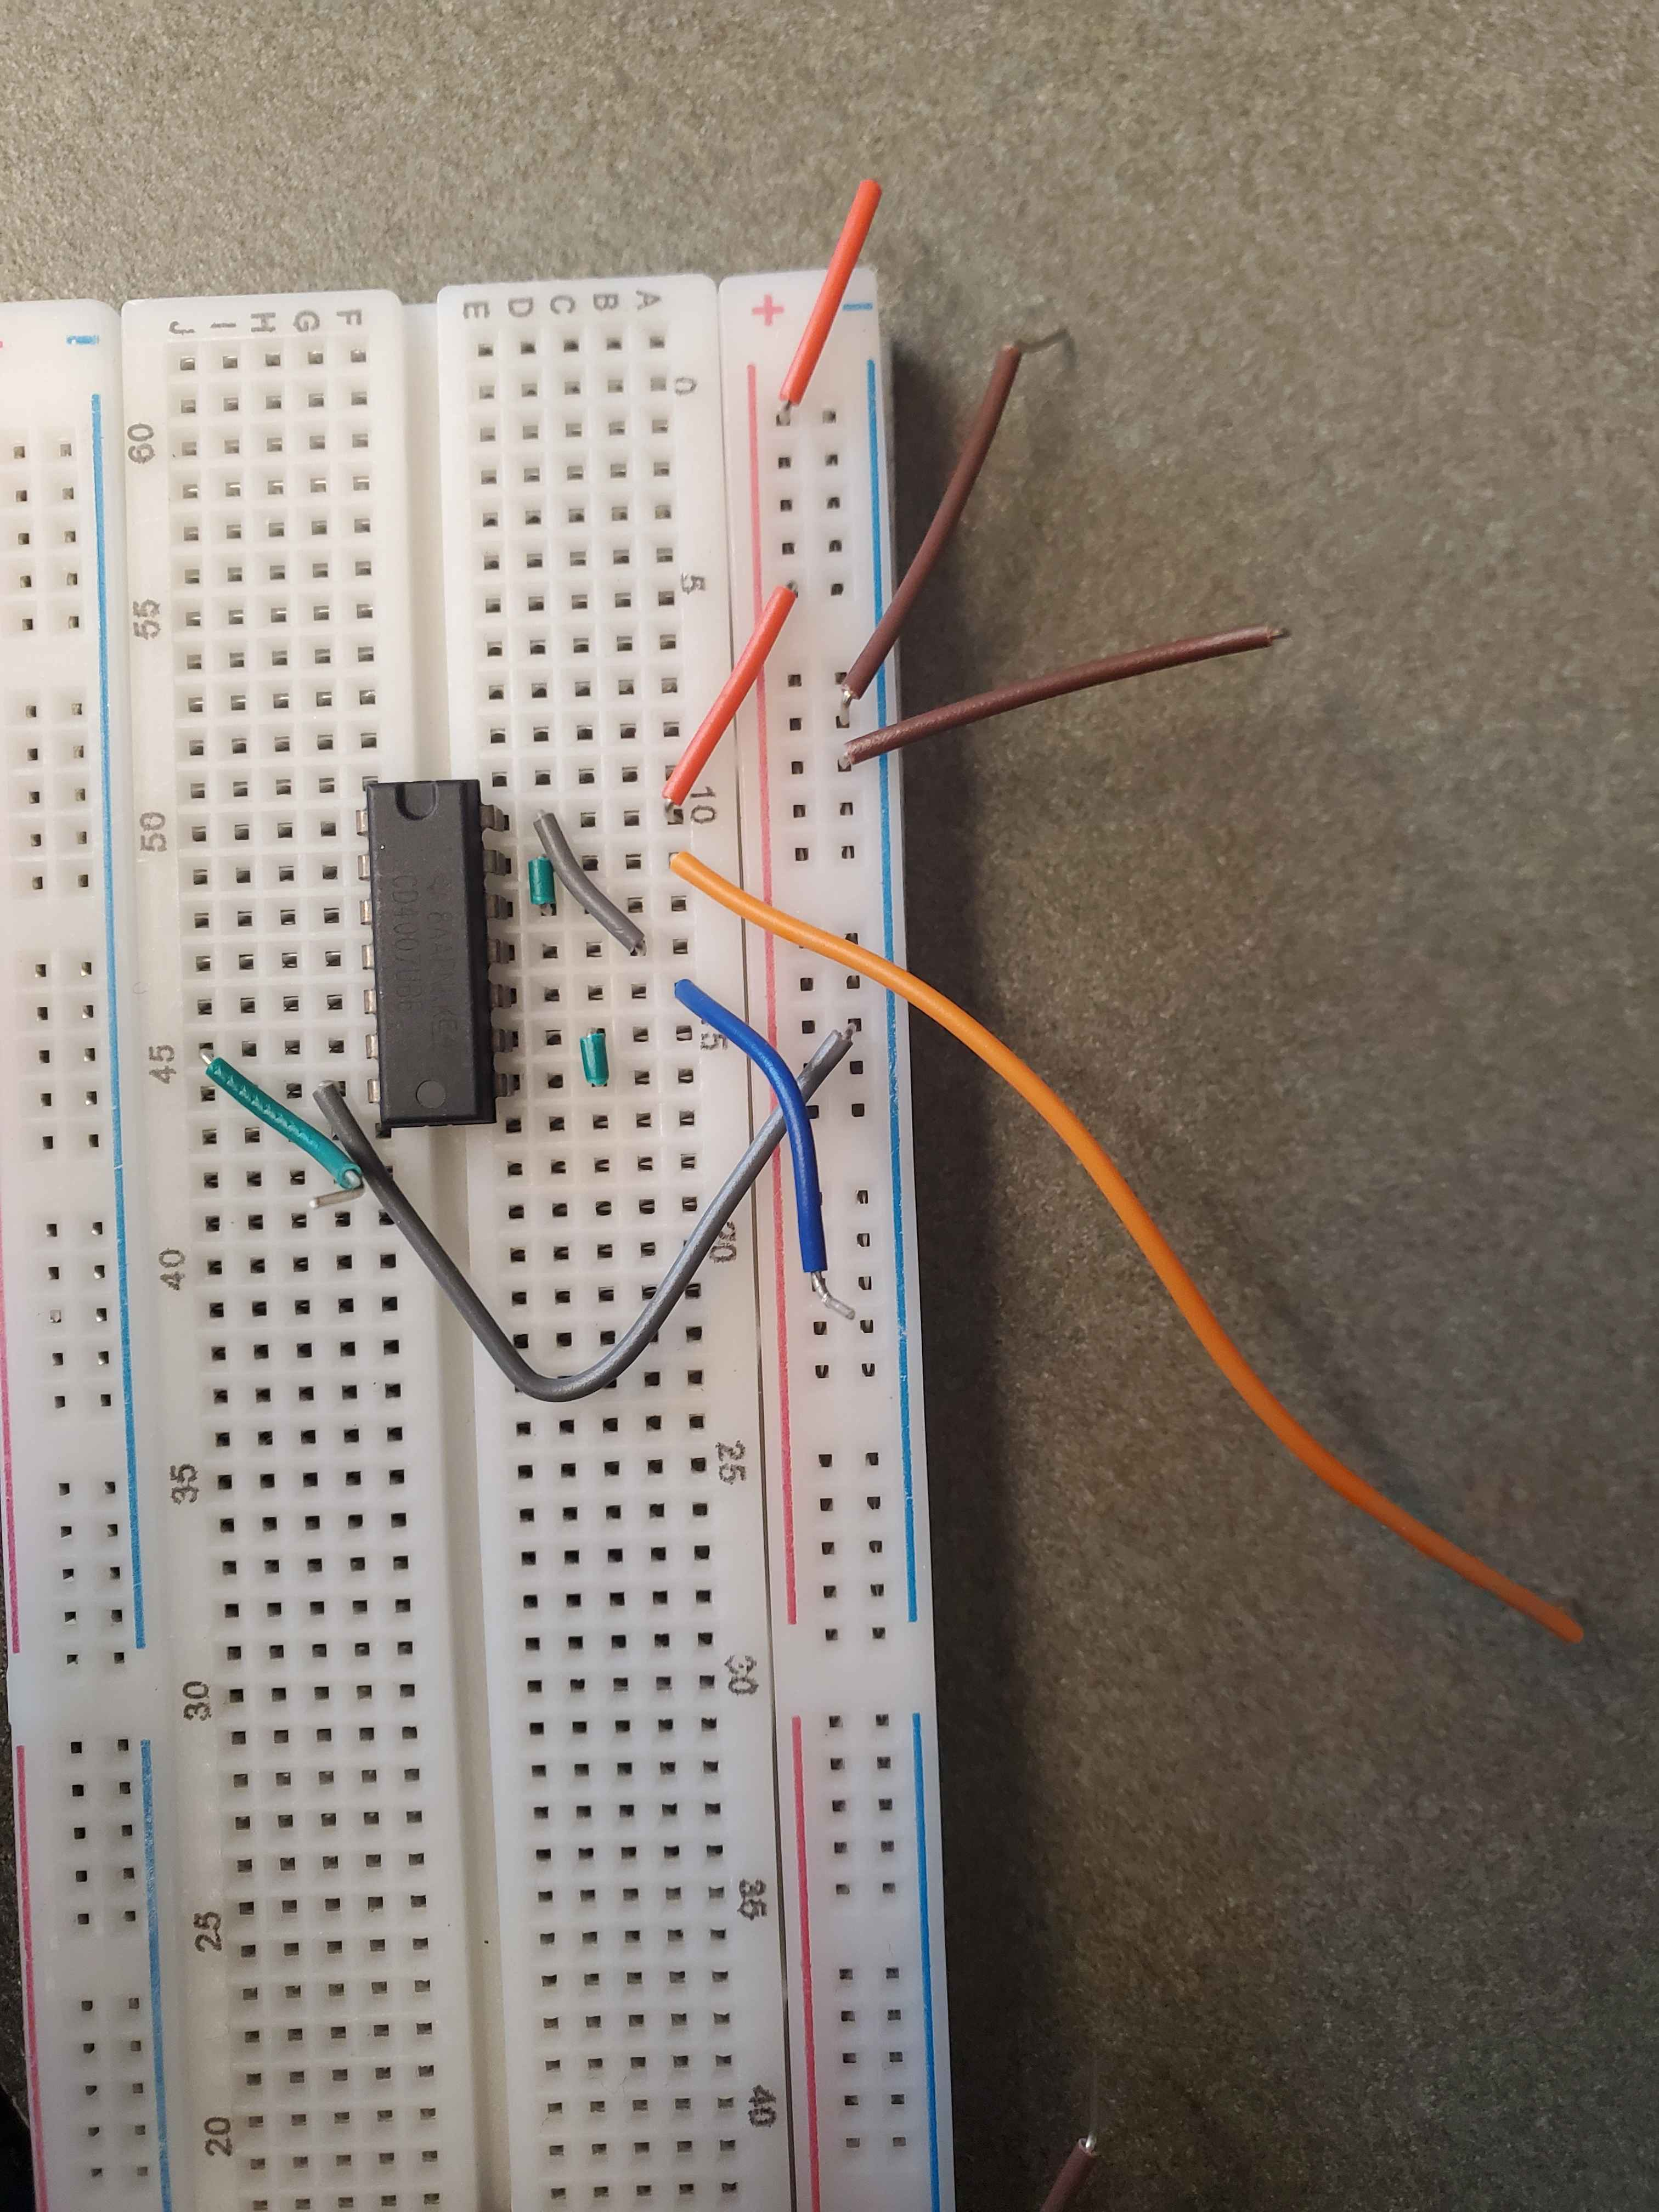
\includegraphics[width=9cm]{20240731_124701}}}
	\subfloat[\centering NAND Gate From CMOS Transistors]{{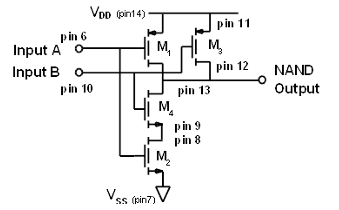
\includegraphics[width=9cm]{NAND_Circuit}}}
\end{figure}

\nsection{Operation}
\emph{Describe a simple description of your NAND gate and how it works transistor by transistor (M1, M2, M3, and M4) = Table 1. 
In the CMOS gate M1 and M3 are PMOSFETs while M2 and M4 are NMOSFETs. Input A controls M1 and M2 while input B controls M3 and M4.}\\\\
When both inputs are off M2 and M4 are off meaning that the output is not connected to ground. At the same time M1 and M3 are on since they are PMOS because the potential difference of the drain is higher than the source. This creates an output of 5V, which is our on-state voltage, and is the same as VDD. \\
When only one input is on one of the PMOS transistors is on and only one of the NMOS transistors is on. This completes the circuit from VDD to the output giving us an on state and a 5V output since the circuit is not completed to ground. Only one of the PMOS transistors needs to be on for this connection because they are connected in parallel so either one of them can connect the output to VDD.
When both inputs are on the NMOS transistors M2 and M4 and the PMOS transistors are off.  This creates a connection between the output and ground giving us an off value of 0V at the output. \\

\nsection{Testing}
\emph{Describe your testing results and insert your Truth Table with voltage outputs and logic levels = ditto.}\\
Our results showed that when the two inputs were set to 5V or “on” we saw our output as 0V or “off”. All other inputs showed the output as 5V which is “on”\\
This high-low relationship for $V_{out}$ is properly represented as an ideal NAND-gate. Seen in the table and truth table, with Spice sim.
\pagebreak

\begin{figure}[hp!]
	\centering
	\subfloat[\centering Gate \& Spice Sim]{{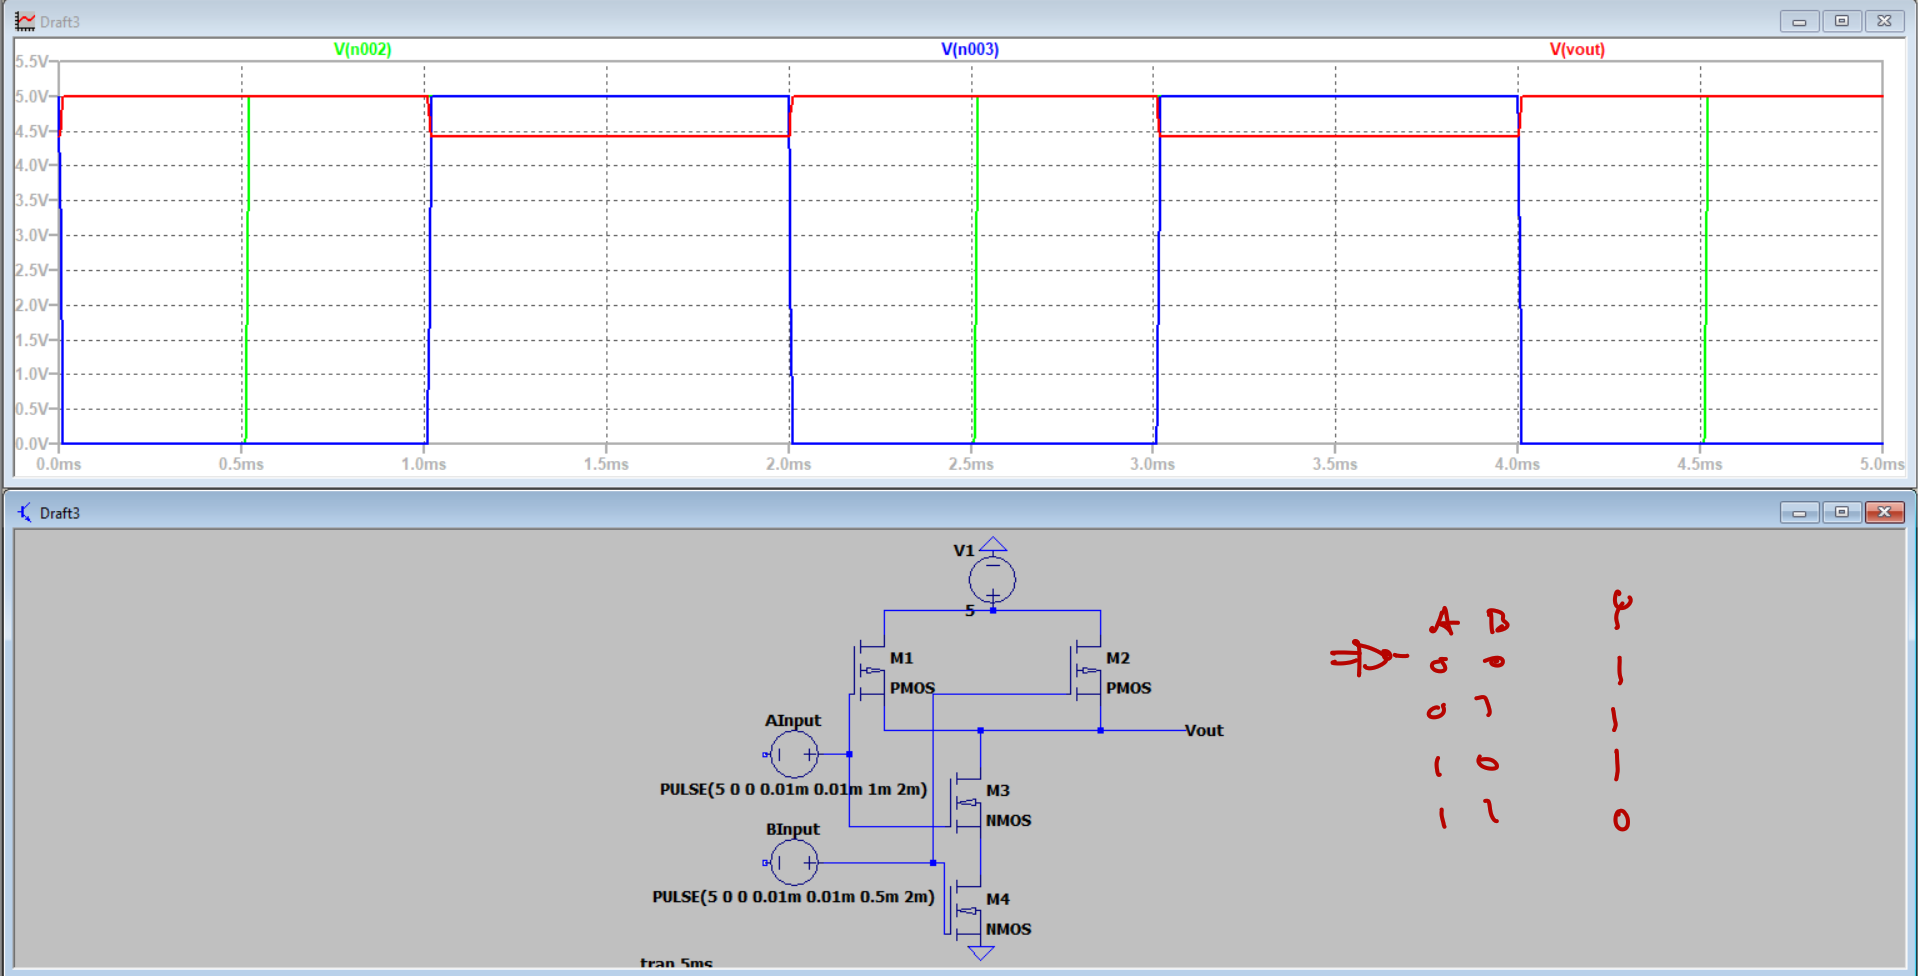
\includegraphics[width=18cm]{Screenshot 2024-08-07 0423451}}}
\end{figure}

\nsection{Describing}
\emph{Describe your test plan and how you would test the NAND gate with two synchronized function generator channels. \textbf{If you have performed this test, paste a scope shot of the output of the NAND gate with each logic level notated.}}\\
Disclaimer: Because the text says "if", we did not.\\\\
When measuring the circuit from the above, which we forgot to take oscilloscope screenshots for - we designed the circuit and developed two separate square-waves that represented high \& low. $V_{out}$, we had 3 voltmeters set up - and alternated between the truth table values above; $2^2$ values.

\begin{figure}[hp!]
	\centering
	\subfloat[\centering NAND Table]{{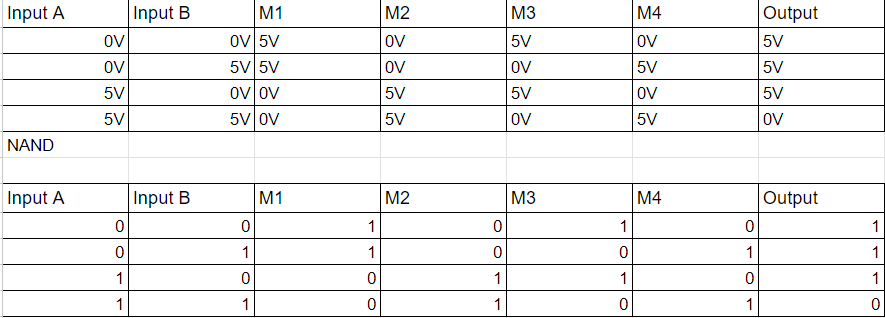
\includegraphics[width=18cm]{Screenshot 2024-08-07 060220}}}
\end{figure}

%NOR Section
\nchapter{CMOS NOR Gate}
\nsection{Design Objective}
In this section we use the CD4007 IC pakage as a NOR logic gate then testing it with two inputs to create a truth table for the transistors.
\nsection{Circuit Diagram and Consturction}
\begin{figure}[hp!]
	\centering
	\subfloat[\centering NOR Circuit Transistors]{{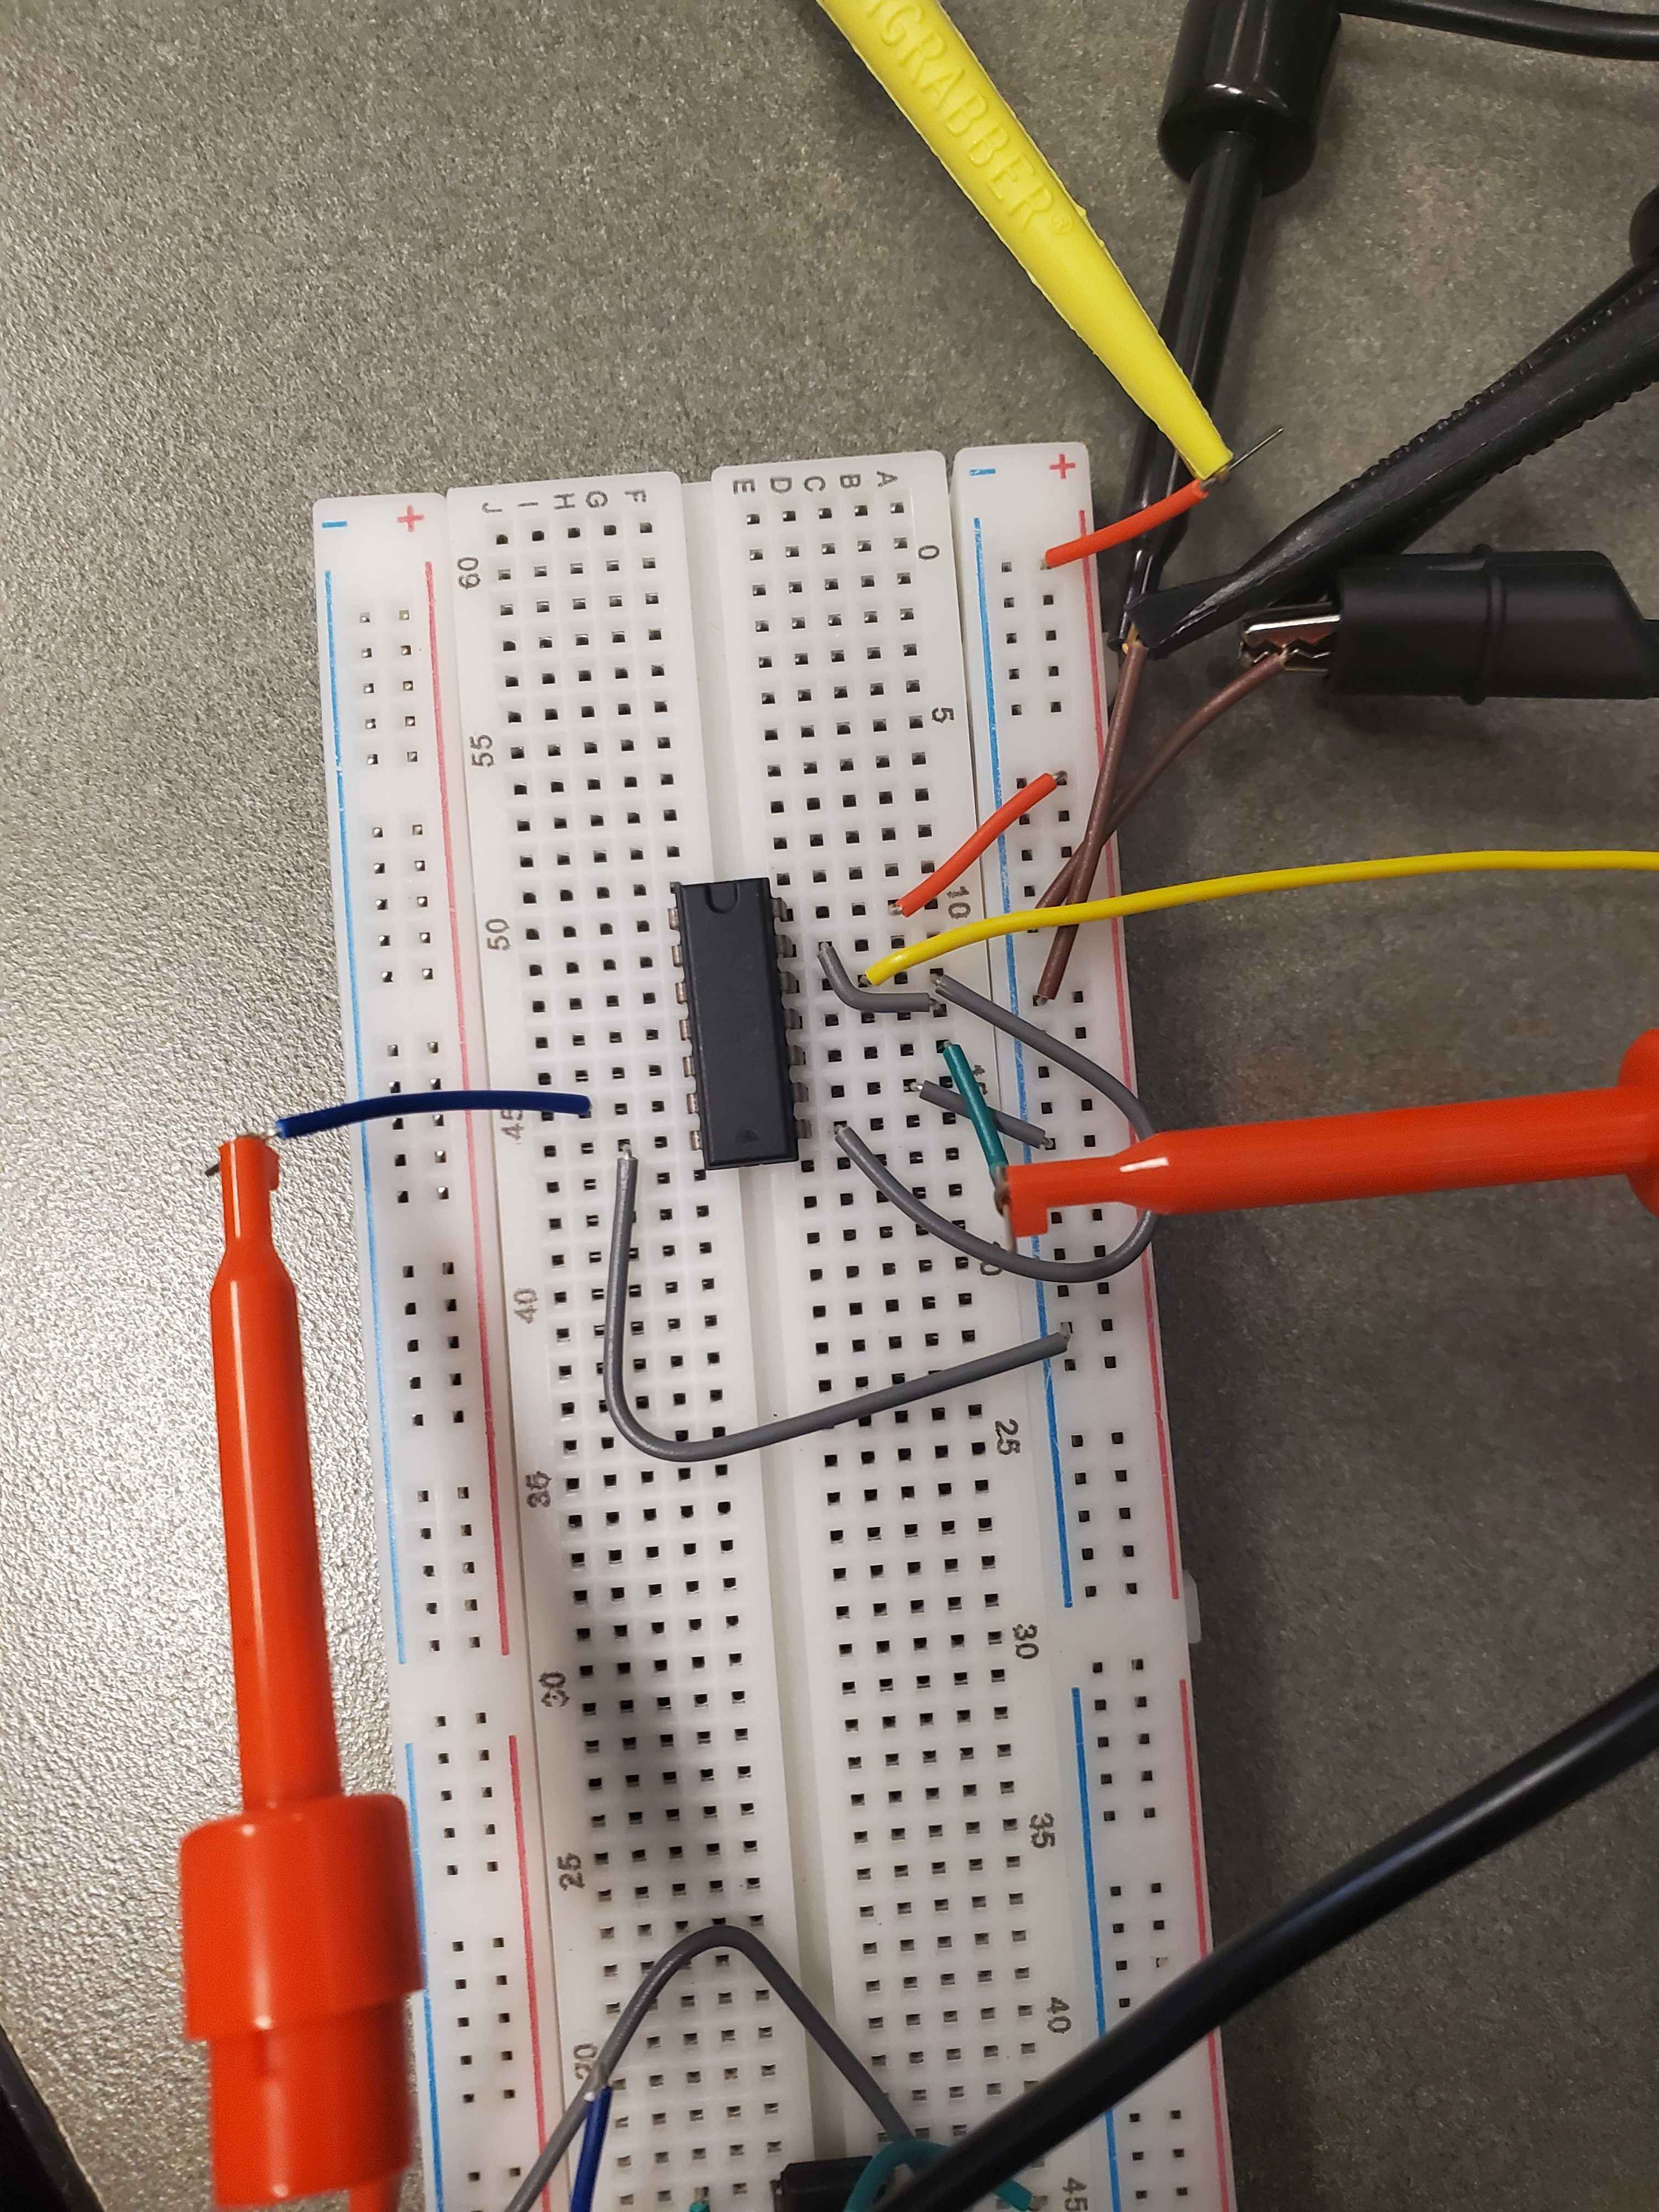
\includegraphics[width=9cm]{20240731_125844}}}
	\subfloat[\centering NOR Gate From CMOS Transistors]{{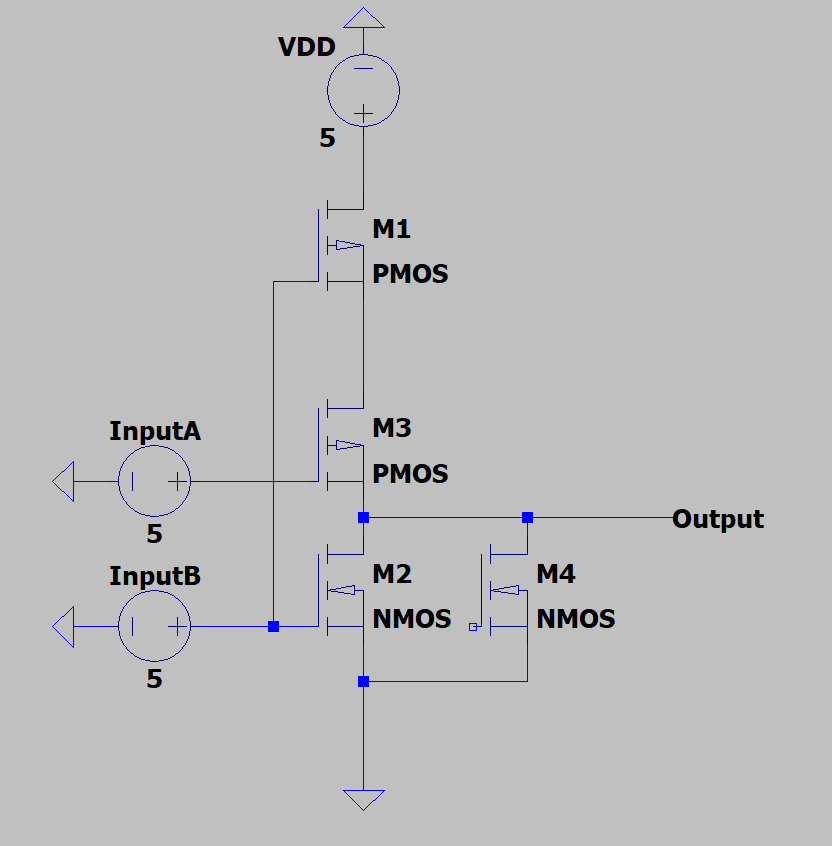
\includegraphics[width=9cm]{3-2_Circuit}}}
\end{figure}

\nsection{Measurements}
\nsection{Design}
Draw your schematic, how you connect parts of the CD4007, and describe a how it works transistor by transistor (M1, M2, M3, and M4) = Table 2 
In the CMOS gate M1 and M3 are PMOSFETs while M2 and M4 are NMOSFETs. Input A controls M3 and M4 while input B controls M1 and M2.\\
When both inputs are off both PMOS transistors are on because there is enough negative difference between drain and source. There is not enough difference for the NMOS transistors to turn on, so they remain in the off state. This makes the output at 5V or in the “on” state because the circuit is connected to VDD through the PMOS network.
When only one input is on one of the PMOS transistors is on and only one of the NMOS transistors is on. This completes the circuit from ground to the output giving us an on state and a 0V. Only one of the NMOS transistors needs to be on for this connection because they are connected in parallel so either one of them can connect the output to ground.\\
When both inputs are on the NMOS transistors M2 and M4 are on and the PMOS transistors are off.  This creates a connection between the output and ground giving us an off value of 0V at the output. \\

\nsection{Static Test}
Fill in states in Table 1, ditto \\\\
Same thing, just with a NOR-Gate. Simple-as.
\nsection{Dynamic Test}
Stimulate the circuit with two square waves, and capture the results.
\newpage
%Spice Sim
\begin{figure}[hp!]
	\centering
	\subfloat[\centering Gate \& Spice Sim]{{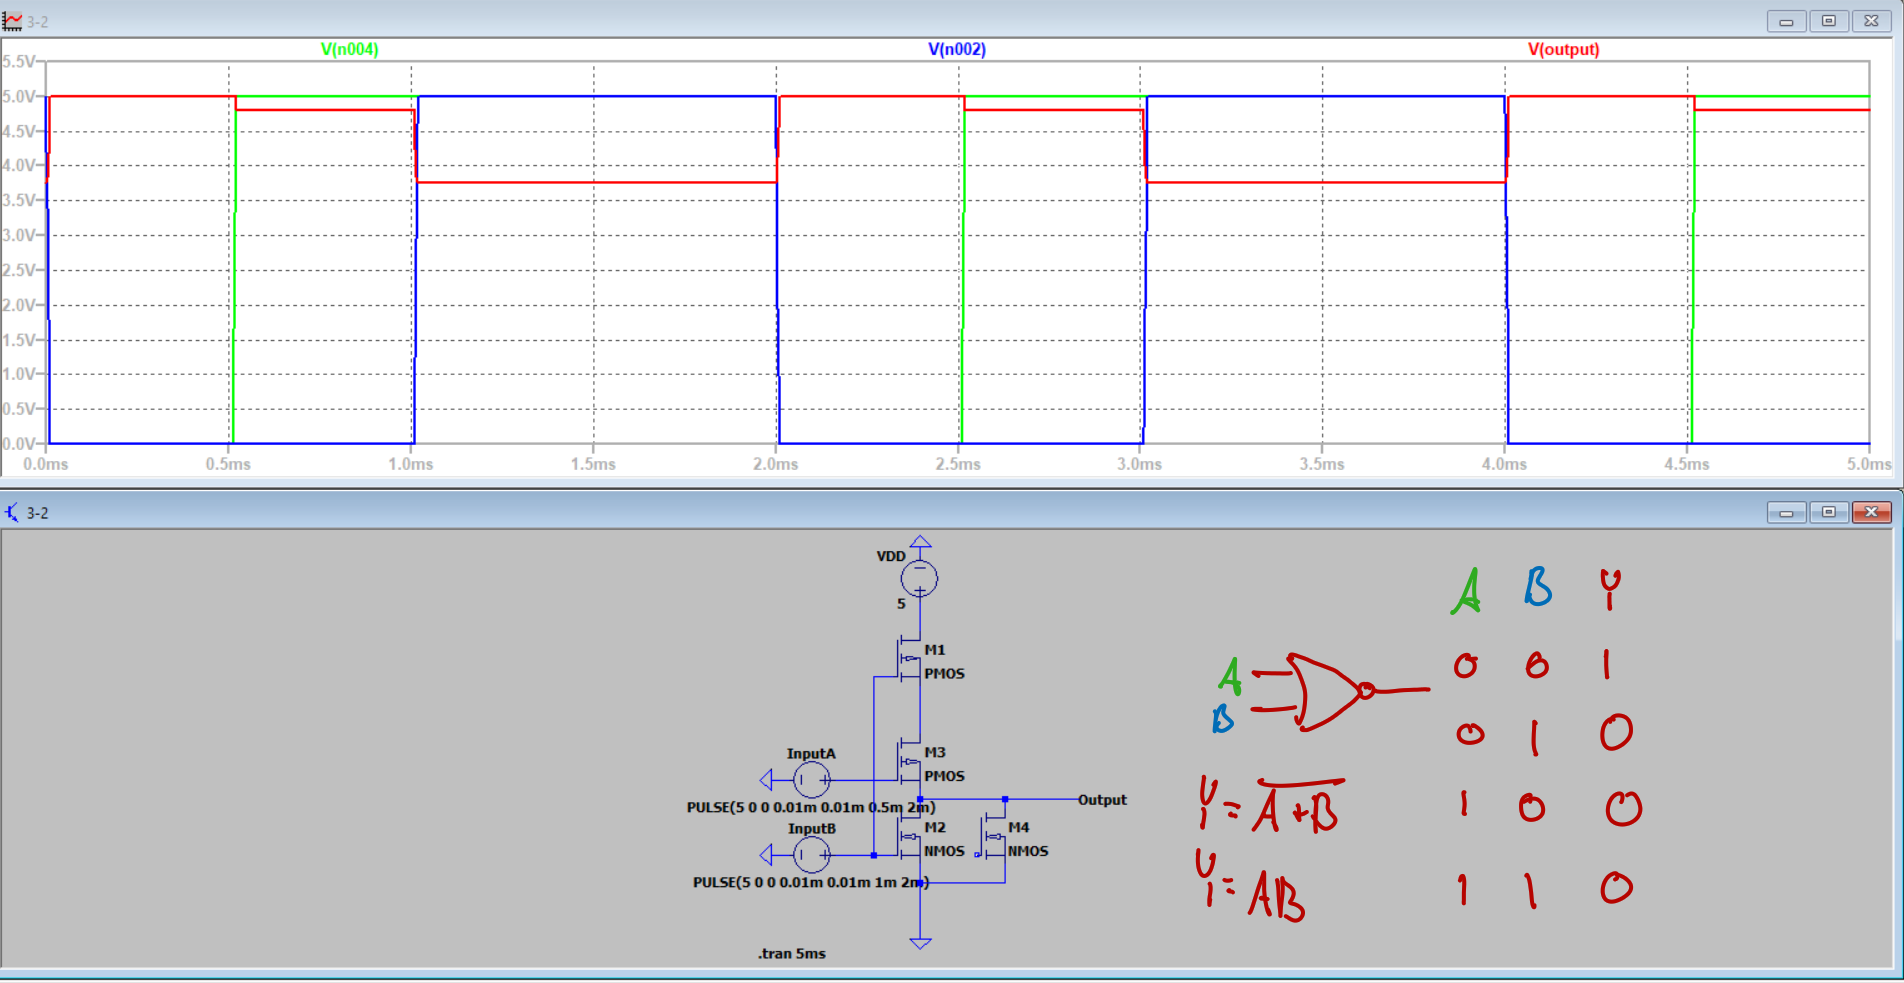
\includegraphics[width=18cm]{Screenshot 2024-08-07 042345}}}
\end{figure}

\nsection{Describing}
\emph{Describe your test plan and how you would test the NOR gate with two synchronized function generator channels.}

\begin{figure}[hp!]
	\centering
	\subfloat[\centering NOR Table]{{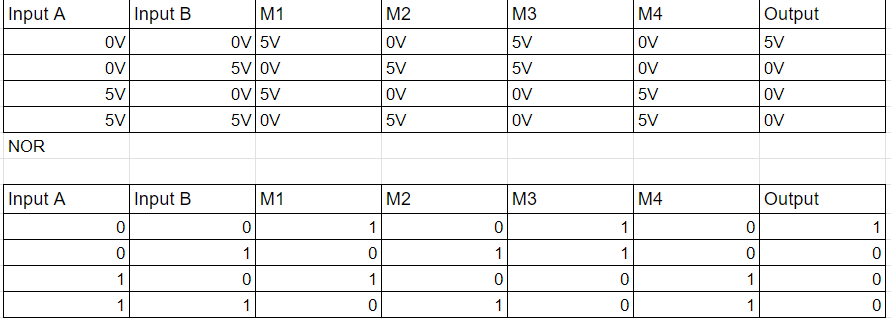
\includegraphics[width=18cm]{Screenshot 2024-08-07 060527}}}
\end{figure}

\newpage
\nsection{Bibliography}
\textbf{Cited:}\\
\begin{itemize}
	\item Lab 1 Manual
	\item Sedra, Adel, and Kenneth Smith. Microelectronic Circuits. S.L., Oxford Univ Press Us, 2019.
\end{itemize}
\begin{figure}[!h]
	\subfloat[It didn't get easier. We just got better.]{
\includegraphics[width=\linewidth]{__penance_arknights_drawn_by_duya_ehouhouohahaha__c12b4a5221fa078ded1b9fc3ca433f0b}}
\end{figure}

\end{document}
